\documentclass[11pt,a4paper]{article}

\usepackage[utf8]{inputenc}
\usepackage{graphicx}
\usepackage[spanish]{babel}
\usepackage{float}				%Para poner las imagenes exactamente donde se me cante las pelotas en caso de quererlo, poniendole [H]
\usepackage{amsmath}
\usepackage{epstopdf}
\usepackage{geometry}
\usepackage{hieroglf}
\usepackage{subcaption}
\usepackage[justification=centering]{caption}
\usepackage[colorinlistoftodos]{todonotes}
\usepackage[colorlinks=true, allcolors=blue]{hyperref}
\geometry{
a4paper,
left=20mm,
right=20mm,
top=25mm,
bottom = 20mm
}
\usepackage{float}
\usepackage{units}
% \usepackage{hyperref}   %Esto es para ir a los links

\newcommand{\rojo}[1]{\textcolor{red}{#1}}    % Comando para escribir texto en rojo




\title{\textbf{Matemática de los Sistemas Biológicos \\ Práctica 1 - Modelos de una sola población}}

\author{
{F. M. Cabrera}
%[1ex] \small{\textit{ Facultad de Ciencias Exactas y Naturales.}} \\
%\small{\textit{Universidad de Buenos Aires. Ciudad Universitaria. Pabellón I. Buenos Aires. Argentina}}
}
\date{\textit{\today}}


% Esto modifica el interlineado
\renewcommand{\baselinestretch}{1}

\graphicspath{{Figuras/}}

\begin{document}

\maketitle

%\thispagestyle{empty} 


\setcounter{page}{1}

%\begin{abstract}


%\end{abstract}
%\vspace*{1cm}

Todo el código implementado en esta practica puede encontrarse \href{https://github.com/cabre94/MSB_IB}{acá}.


\section*{Ejercicio 1 - Modelo de Goodwin}

Tenemos un mecanismo de regulación de la expresión de un gen, descripto por
\begin{align}
    \frac{dm}{dt} &= \alpha_m g_{R}\left(p\right) - \beta_m m \\
    \frac{de}{dt} &= \alpha_e m - \beta_e e \\
    \frac{dp}{dt} &= \alpha_p e - \beta_p p
\end{align}
donde $m$ es la concentración del mRNA, que produce la enzima $e$, la cual contribuye a la producción de una proteína $p$. La regulación está controlada por la proteína, con una función de represión de la forma:
\begin{equation}
    g_R \left(p\right) = \frac{a}{b+cp^{h}}.
    \label{eq:represion}
\end{equation}

En la Fig. \ref{ej1:concentraciones_barrido_h} se observan los resultados de la simulación numérica realizada para distintos valores del parámetro de Hill $h$, fijando los valores del resto de los parámetros a $\alpha_m = \alpha_e = \alpha_e =1$, $a=b=c=1$ y $\beta_m = \beta_e = \beta_p = 0.1$. Luego de un periodo transitorio, se observa que para $h=8$ y $h=12$ las oscilaciones son sostenidas, con una mayor amplitud para $h=12$, mientras que para $h=6$ las oscilaciones son amortiguadas y terminan desapareciendo.

\begin{figure}[htb!]
    \centering
    \begin{subfigure}[b]{0.42\textwidth}
        \includegraphics[width=\textwidth]{../ej1_Resultados/h=6_Concentraciones.pdf}
    \end{subfigure}
    \begin{subfigure}[b]{0.42\textwidth}
        \includegraphics[width=\textwidth]{../ej1_Resultados/h=8_Concentraciones.pdf}
    \end{subfigure}
    \begin{subfigure}[b]{0.42\textwidth}
        \includegraphics[width=\textwidth]{../ej1_Resultados/h=12_Concentraciones.pdf}
    \end{subfigure}
    \caption{Evolución de las concentraciones de mRNA, proteína y enzima para distintos valores del parámetro de Hill $h$. Luego de un periodo transitorio, se observa que para $h=8$ y $h=12$ las oscilaciones son sostenidas, con una mayor amplitud para $h=12$, mientras que para $h=6$ las oscilaciones son amortiguadas y terminan desapareciendo.}
    \label{ej1:concentraciones_barrido_h}
\end{figure}

En la Fig. \ref{ej1:concentraciones_barrido_h_estacionario} se observan los mismos resultados que en la Fig. \ref{ej1:concentraciones_barrido_h} pero para tiempos mas largos, de manera de observar en detalle el periodo estacionario del sistema. Se observa que para $h=7$ las oscilaciones continúan disminuyendo su amplitud, al igual que para $h=8$ (aunque puede suceder que aun no se haya alcanzado el estado estacionario), pero para $h=10$ y $h=14$ las oscilaciones ya son sostenidas.

\begin{figure}[htb!]
    \centering
    \begin{subfigure}[b]{0.42\textwidth}
        \includegraphics[width=\textwidth]{../ej1_Resultados/m_estacionario.pdf}
    \end{subfigure}
    \begin{subfigure}[b]{0.42\textwidth}
        \includegraphics[width=\textwidth]{../ej1_Resultados/p_estacionario.pdf}
    \end{subfigure}
    \begin{subfigure}[b]{0.42\textwidth}
        \includegraphics[width=\textwidth]{../ej1_Resultados/e_estacionario.pdf}
    \end{subfigure}
    \caption{Estado estacionario de las concentraciones de mRNA, proteína y enzima para distintos valores del parámetro de Hill $h$. Se observa que para $h=7$ las oscilaciones continúan disminuyendo su amplitud, al igual que para $h=8$ (aunque puede suceder que aun no se haya alcanzado el estado estacionario), pero para $h=10$ y $h=14$ las oscilaciones ya son sostenidas.}
    \label{ej1:concentraciones_barrido_h_estacionario}
\end{figure}

Luego, utilizando un valor de $h=10$ en el cual se observaran oscilaciones, se busco estudiar el efecto en la dinámica del sistema al aumentar la degradación $\beta$ de las distintas concentraciones. El resto de parámetros $\alpha_i$ y $a$, $b$ y $c$ se mantuvieron iguales y se utilizo el mismo valor de la degradación tanto para el mRNA, la proteína y la enzima. En la Fig. \ref{ej1:concentraciones_barrido_b} se observan los resultados obtenidos para valores de $\beta$ iguales a $0.1$, $0.5$ y $1$. Al aumentar el valor de $\beta$ a $0.5$, primero se observa que las oscilaciones aumentan tanto su frecuencia como su amplitud respecto a las oscilaciones observadas para $\beta=0.1$. Luego, al continuar aumentando $\beta$, se observa que las oscilaciones desaparecen para todas las concentraciones.

\begin{figure}[htb!]
    \centering
    \begin{subfigure}[b]{0.49\textwidth}
        \includegraphics[width=\textwidth]{../ej1_Resultados/b=0.1_Barrido.pdf}
    \end{subfigure}
    \begin{subfigure}[b]{0.49\textwidth}
        \includegraphics[width=\textwidth]{../ej1_Resultados/b=0.5_Barrido.pdf}
    \end{subfigure}
    \begin{subfigure}[b]{0.49\textwidth}
        \includegraphics[width=\textwidth]{../ej1_Resultados/b=1_Barrido.pdf}
    \end{subfigure}
    \caption{Evolución de las concentraciones de mRNA, proteína y enzima para distintos valores del parámetro $\beta$, tomando $h=10$. Al aumentar el valor de $\beta$ a $0.5$, primero se observa que las oscilaciones aumentan tanto su frecuencia como su amplitud respecto a las oscilaciones observadas para $\beta=0.1$. Luego, al continuar aumentando $\beta$, se observa que las oscilaciones desaparecen para todas las concentraciones.}
    \label{ej1:concentraciones_barrido_b}
\end{figure}

\section*{Ejercicio 2}
\graphicspath{{Figuras/}}

Se busco estudiar una generalización del problemas de XOR para $N$ entradas, en donde la salida esperada es el producto de todas las componentes de la entrada. La arquitectura utilizada consistió en una capa oculta de $N'$ neuronas con una función de activación \texttt{tanh}, seguida de una capa de salida de 1 neurona tambien con activacion \texttt{tanh}. Debido a que la cantidad de datos de entrada es igual a $2^{N}$ y era de interés estudiar los casos en donde $N>N'$ y $N<N'$, se fijo $N$ a un valor de 5 y se entreno la red para distintos valores de $N'$: 1, 3, 5, 7, 9 y 11, en todos ellos durante 5000 épocas.

\begin{figure}[h!]
    \centering
    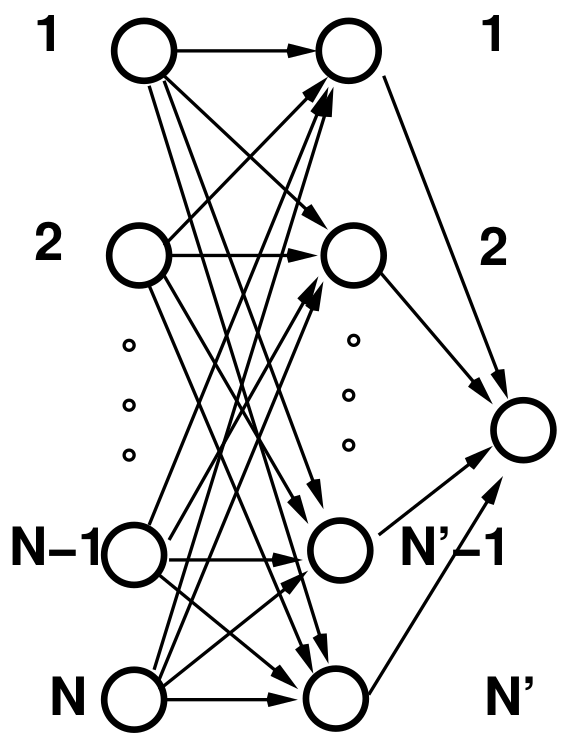
\includegraphics[width=0.3\textwidth]{Figuras/ejer_2_NN1.png}
    \caption{Esquema de la arquitectura utilizada para resolver el problema del XOR generalizado.}
    \label{02:fig:Arquitectura}
\end{figure}

En la Figura \ref{fig:2_Resultados} se observan los resultados obtenidos para la función de costo y \textit{accuracy} en cada uno de los casos. En caso de que $N'>N$, los resultados son similares a los del ejercicio anterior, ya que en una pequeña cantidad de épocas se obtiene un 100\% de precisión. La situación se vuelve mas problemática al disminuir $N'$, en donde se observa que para $N'=N=5$ el aprendizaje de la red nunca alcanza una precisión total e incluso no mejora de manera monótona conforme avanzan las épocas. Los resultados son incluso peores cuando $N'<N$, en donde se requieren muchas mas épocas para que la red aprenda e incluso para $N'=1$ nunca se logra alcanzar un valor de \textit{accuracy} no nulo. Este problema es esperable, ya que el valor de $N'$ determina las dimensiones de las matrices de pesos de cada una de las capas. Al disminuir $N'$, menor sera la cantidad de componentes de estas matrices, con lo cual deberá ajustar una gran cantidad de datos de entrada ($2^{N}$) con menos grados de libertad, que, en caso de ser demasiado pocos, se presentara un problema de underfitting y la red no mejorara sus resultados.


\begin{figure}[h!]
    \centering
    \begin{subfigure}[h]{0.49\textwidth} 
        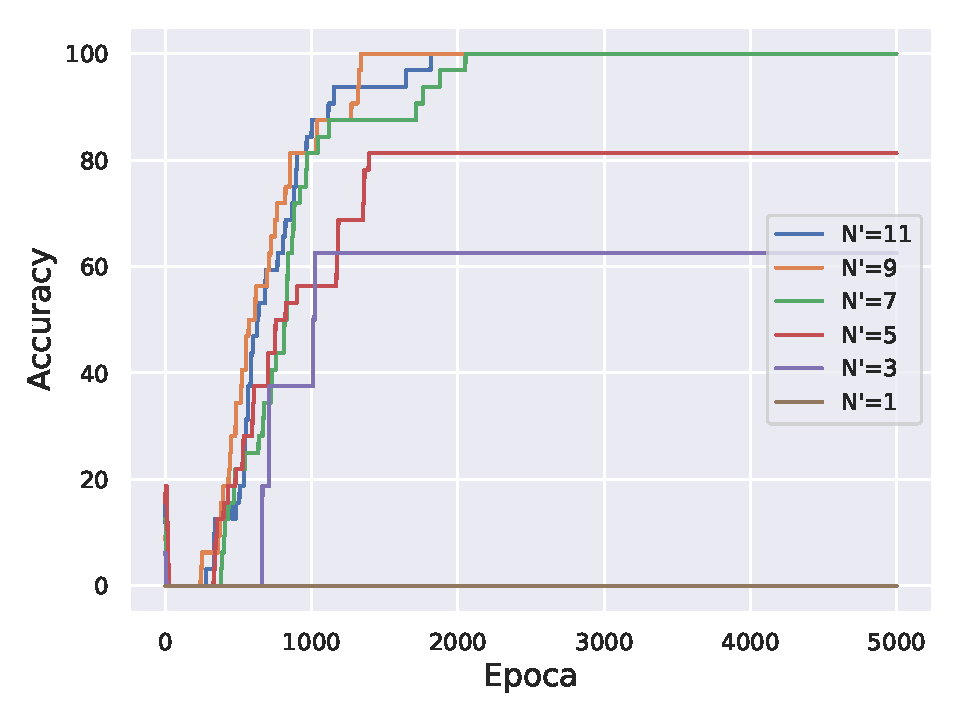
\includegraphics[width=\textwidth]{Figuras/ej2/Acc.pdf}
    \end{subfigure}       
    \begin{subfigure}[h]{0.49\textwidth} 
        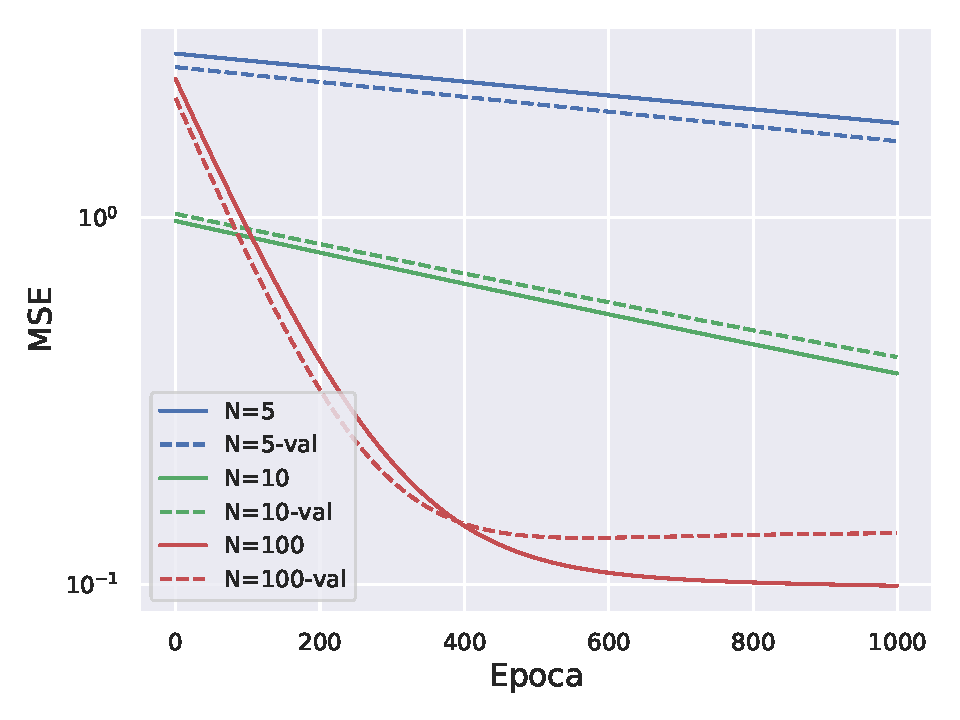
\includegraphics[width=\textwidth]{Figuras/ej2/Loss.pdf}
    \end{subfigure}
    \caption{Función de costo MSE y \textit{accuracy} para el entrenamiento de 6 modelos independientes variando la cantidad de neuronas de la capa oculta, utilizando la arquitectura propuesta en Fig. \ref{fig:1_Arquitecturas}.}
    \label{fig:2_Resultados}
\end{figure}
\section*{Ejercicio 3}
\graphicspath{{Figuras/}}

En este ejercicio se busco obtener un histograma de la tasa de disparo dependiente del tiempo $r(t)$. Esta se obtiene calculando el promedio de spikes en las 128 realizaciones para cada intervalo de tiempo, en este caso $0.1\,\text{ms}$, y luego dividiendo por dicho intervalo. El resultado obtenido puede observarse en la Figura \ref{03:fig:rt}. 

\begin{figure}[h!]
    \centering
    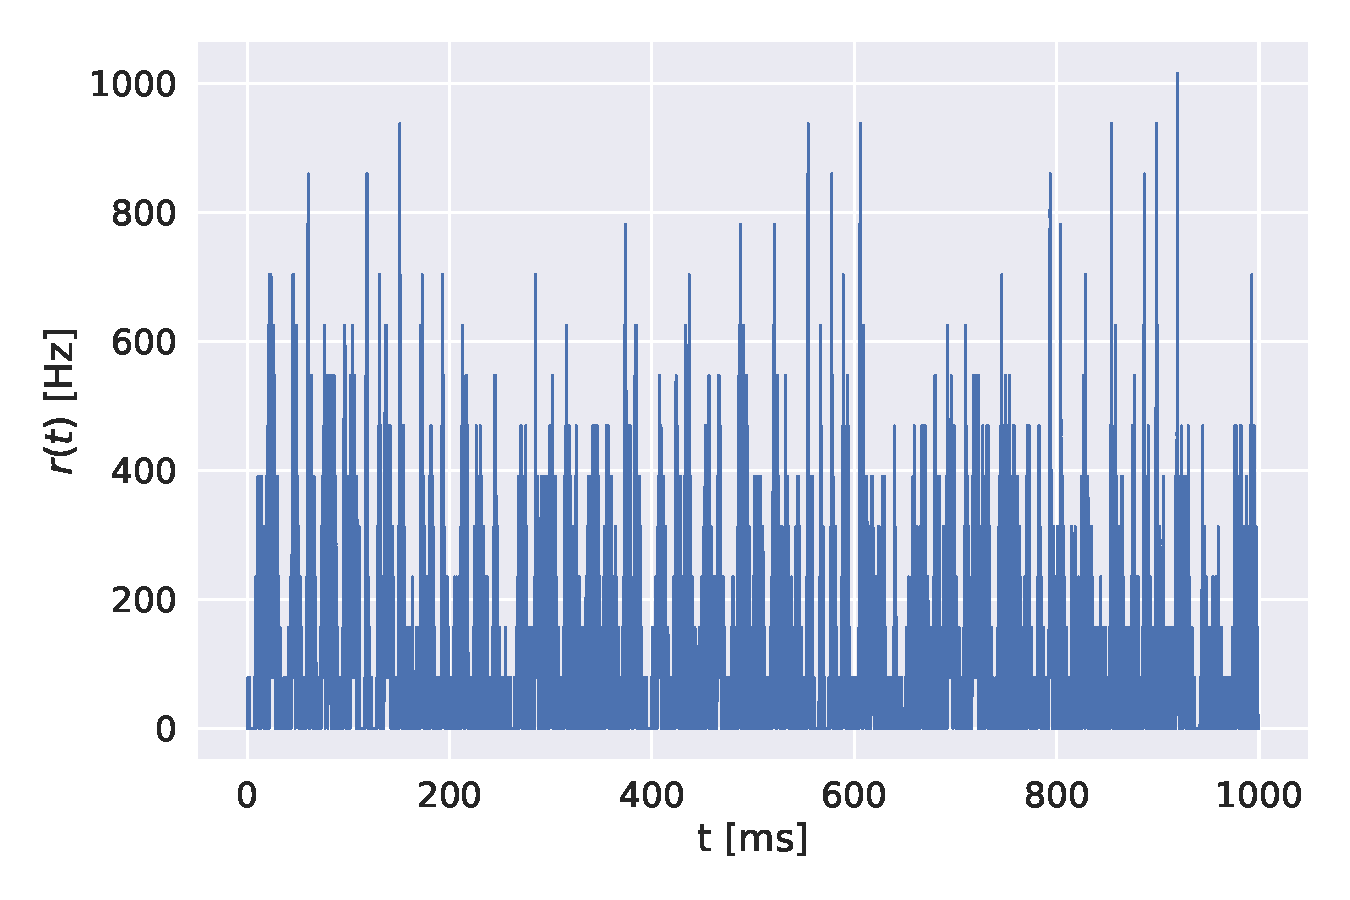
\includegraphics[width=0.75\textwidth]{3_rt.pdf}
    \caption{Histograma de la tasa de disparo $r(t)$ como función del tiempo, promediada para las 128 realizaciones.}
    \label{03:fig:rt}
\end{figure}
\section*{Ejercicio 4}
\graphicspath{{Figuras/ej_04/}}

Tenemos una especie con un ciclo de vida anual en la que cada individuo produce $r$ descendientes y luego muere, cuya evolución describimos como
\begin{equation}
    N_{t+1} = r N_{t}
    \label{04_Modelo}
\end{equation}
y en donde $r$ obedece a una distribución de Poisson con media $1.7$\footnote{No me queda super claro del enunciado, pero estoy asumiendo que en cada iteracion el valor de $r$ se modifica aleatoriamente según la distribución descripta.}.

Simulando el sistema con 1 solo individuo como condición inicial, se observan tres comportamientos distintos según $r$ sea $0$, $1$ o mayor que $1$. Estos tres comportamientos pueden observarse en la Figura \ref{04_Simulacion}. Para rachas en donde $r>1$, la población crece en cada ciclo, mientras que si $r=1$ la población se mantiene, observándose escalones en la evolución de la especie, como se observa para $t$ entre 3 y 6 en la figura. Por último, para el primer ciclo en donde $r=0$, la población se extingue y sin importar el valor de $r$ para iteraciones posteriores, se mantiene en $0$. 

\begin{figure}[h!]
    \centering
    \includegraphics[width=0.6\textwidth]{Simulacion1.pdf}
    \caption{Evolución del sistema para el modelo \ref{04_Modelo} en donde $r$ obedece a una distribución de Poisson con media $1.7$. Se observan tres comportamiento cualitativamente distintos. Para $r>1$, la población crece, para $r=1$ la población se mantiene y se observan escalones en la evolución del sistema y por último para $r=0$ la especie se extingue.}
    \label{04_Simulacion}
\end{figure}

En general, estudiando la evolución del sistema a lo largo de 20 ciclos, se observa que la especie no logra sobrevivir. Veamos porque sucede esto. La densidad de probabilidad es $\frac{e^{-\lambda}\lambda^{k}}{k!}$, con lo cual la probabilidad de que en un ciclo $r$ sea $0$ es $e^{-1.7}\approx0.183$. Entonces, la probabilidad de que $r$ sea distinto de cero en 20 ciclos es $(1-e^{-1.7})^{20}\approx0.01769$. Es decir que la probabilidad de que la especie sobreviva luego de 20 ciclos es de $1.769\%$. Generando cien millones de simulaciones, se obtuvo que en un $1.767\%$ la especie logra sobrevivir, corroborando el calculo previamente descripto. 
\section*{Ejercicio 5 - Metapoblaciones de presa y depredador}

De las diapositivas de clase, tomamos el modelo de dos especies compitiendo, en donde la especie $p_1$ es mejor colonizadora y desplaza a la especie $p_2$ (donde $p_i$ es la fracción de parches ocupados). $c_i$ son las tasas de colonización de cada especie y $c_i$ las tasas de extinción o probabilidad de que un parche quede vacio
\begin{align}
    \dot{p_1} &= c_1 p_1 \left(1-p_1\right) -e_1 p_1 \\ 
    \dot{p_2} &= c_2 p_2 \left(1-p_1-p_2\right) -e_2 p _2 - c_1 p_1 p_2 
\end{align}

Los puntos fijos del sistema son $\left(0,0\right)$, $\left[0, 1-\frac{e_2}{c_2}\right]$, $\left(1-\frac{e_1}{c_1}\right)$ y $\left(1-\frac{e_1}{c_1}, \frac{e_1}{c_1} + \frac{c_1-e_2-e_1}{c_2}\right)$. En el punto fijo $\left(0,0\right)$ no hay ninguna especie. En $\left[0, 1-\frac{e_2}{c_2}\right]$ tenemos solo tenemos a la presa como especie sobreviviente y es un caso posible solo si $\frac{e_2}{c_2} < 1$. Por otro lado, $\left(1-\frac{e_1}{c_1}\right)$ es un equilibrio donde solo hay depredador y es un equilibrio posible si $\frac{e_1}{c_1} < 1$. 

Por ultimo, para el equilibrio que existe coexistencia $\left(1-\frac{e_1}{c_1}, \frac{e_1}{c_1} + \frac{c_1-e_2-e_1}{c_2}\right)$, tenemos primero que debe cumplirse $\frac{e_1}{c_1} < 1$ para que haya población de depredador. Por otro lado, si queremos que sea una equilibrio estable, los dos autovalores deben ser negativos, con lo cual calculando el Jacobiano obtenemos la condición
\begin{equation}
    c_2 > c_1 \left(\frac{c_1 + e_2 + e_1}{e_1}\right).
\end{equation}
\section*{Ejercicio 6}
\graphicspath{{Figuras/ej_06/}}

Tenemos el modelo para describir el efecto Allee
\begin{equation}
    \frac{dN}{dt} = f(N) = r N \left[ 1 - \frac{N}{K} \right] \left[ \frac{N}{A} -1 \right]
\end{equation}
de donde planteando que $f(N) = 0$ obtenemos que los puntos fijos son 0, $A$ y $K$. Para estudiar la estabilidad calculamos la derivada $f'(N)$ obteniendo
\begin{equation}
    f'(N) = r \left[ 1-\frac{N}{K} \right] \left[ \frac{N}{A} -1 \right] + \frac{rN}{A} \left[ 1 - \frac{N}{K} \right] - \frac{rN}{K} \left[ \frac{N}{A}-1\right]
\end{equation}
que evaluando en los puntos fijos obtenidos, tenemos que
\begin{equation}
    f'(N=0) = -r; \indent f'(N=A)=r\left[1-\frac{A}{K}\right]; \indent f'(N=K)=r\left[1-\frac{K}{A}\right]. 
\end{equation}

Para seguir avanzando con el análisis, tomamos el caso en que $r>0$ y $0<A<K$. En esta situación, los puntos fijos en $0$ y $K$ son puntos fijos estables, mientras que el punto fijo en $A$ es inestable. En la Figura \ref{06_Simulacion} se observa la simulación obtenido del sistema para distintas condiciones iniciales. En esta figura se observan dos regímenes, uno en el intervalo $[0,A)$ en donde el sistema evoluciona al equilibrio estable en $0$ y la población se extingue y otro en $[A,\infty)$ en donde el sistema evoluciona al equilibrio estable en $K$ y la población sobrevive. En la Figura \ref{06_Funcion_y_raices} se observa la función que determina la evolución del sistema indicando con flechas sobre el eje de abscisa la evolución del sistema.

\begin{figure}[hb!]
    \centering
    \begin{subfigure}[b]{0.49\textwidth}
        \includegraphics[width=\textwidth]{Simulacion.pdf}
        \caption{}
        \label{06_Simulacion}
    \end{subfigure}
    % \hfill
    \begin{subfigure}[b]{0.49\textwidth}
        \includegraphics[width=\textwidth]{f.pdf}
        \caption{}
        \label{06_Funcion_y_raices}
    \end{subfigure}
    \caption{En la Figura (a) se observa la evolución del sistema para distintas condiciones iniciales, tomando $r>0$ y $0<A<K$. Se observan dos regímenes, uno en el intervalo $[0,A)$ en donde el sistema evoluciona al equilibrio estable en $0$ y la población se extingue y otro en $[A,\infty)$ en donde el sistema evoluciona al equilibrio estable en $K$ y la población sobrevive. En la Figura (b) se observa la función que determina la evolución del sistema indicando con flechas sobre el eje de abscisa la evolución del sistema. }
    \label{06_ejercicio}
\end{figure}

La diferencia que puede observarse respecto a la ecuación logística, ademas de la aparición de un nuevo punto fijo en $A$, es que la aparición de este nuevo punto fijo genera un cambio en la estabilidad del punto fijo en $0$, el cual es inestable en la ecuación logística mientras que en este caso dicho punto es estable (para $r>0$). De esta forma, como ya se remarco previamente, existe un numero mínimo ($A$) para la población para que la supervivencia sea posible.

En caso de que $0<K<A$, las estabilidades de los puntos fijos en $A$ y $K$ cambian, pero también cambian sus posiciones, con lo cual la situación es análoga a cuando $0<A<K$.
%Por otro lado, si $r<0$, la estabilidad de todos los puntos fijos se invierte


\bibliographystyle{acm}
\bibliography{biblio}

\end{document}



